
% Include LaTeX packages
\documentclass[conference]{styles/acmsiggraph}
\usepackage{comment} % enables the use of multi-line comments (\ifx \fi)
\usepackage{fullpage}
\usepackage{enumitem}
\usepackage{amsmath,amsthm,amssymb}
\usepackage{listings}
\usepackage{graphicx}
\usepackage{etoolbox}
\usepackage{verbatim}
\usepackage{minted}
\usepackage[dvipsnames]{xcolor}
\usepackage{fancyvrb}
\usepackage{hyperref}
\usepackage{menukeys}
\usepackage{titlesec}
\usepackage{csquotes}
\usepackage{placeins}
\usepackage{algorithm} 
\usepackage{cases} 
\usepackage{algpseudocode}
\usepackage{unicode-math}
\newcommand{\?}{\stackrel{?}{=}}
\renewcommand\qedsymbol{$\blacksquare$}

% Set additional LaTeX options
\setlength{\parskip}{.8mm}
\setcounter{MaxMatrixCols}{20}
\hypersetup{
	colorlinks=true,
	urlcolor=[rgb]{0.97,0,0.30},
	anchorcolor={0.97,0,0.30},
	linkcolor=black,
	filecolor=[rgb]{0.97,0,0.30},
}

% Define title, author, and affiliation information
\title{\huge PSET 4 \\ \LARGE {CS124: Data Structures and Algorithms \\ Prof. Mitzenmacher}}
\author{\Large Dhilan Ramaprasad \\ dhilanramaprasad@college.harvard.edu}
\pdfauthor{Student Name}

% Redefine \VerbatimInput
\RecustomVerbatimCommand{\VerbatimInput}{VerbatimInput}%
{fontsize=\footnotesize,
 %
 frame=lines, % top and bottom rule only
 framesep=2em, % separation between frame and text
 rulecolor=\color{Gray},
 %
 label=\fbox{\color{Black}\textbf{OUTPUT}},
 labelposition=topline,
 %
 commandchars=\|\(\), % escape character and argument delimiters for commands within the verbatim
 commentchar=* % comment character
}

% Set addditional formatting options
\titlespacing*{\section}{0pt}{5.5ex plus 1ex minus .2ex}{2ex}
\titlespacing*{\subsection}{0pt}{3ex}{2ex}
\setcounter{secnumdepth}{4}
\renewcommand\theparagraph{\thesubsubsection.\arabic{paragraph}}
\newcommand\subsubsubsection{\paragraph}

% Define a convenient norm symbol
\newcommand{\norm}[1]{\left\lVert#1\right\rVert}
\renewcommand{\vec}[1]{\mathbf{#1}}

% Define a macro for hiding answers
\newbool{hideanswers} \setbool{hideanswers}{false}
\newenvironment{answer}{}{}
\ifbool{hideanswers}{\AtBeginEnvironment{answer}{\comment} %
\AtEndEnvironment{answer}{\endcomment}}{}

% Define text formatting for points and normals
\newcommand{\points}[1]{\hfill \normalfont{(\textit{#1pts})}}
\newcommand{\pointsin}[1]{\normalfont{(\textit{#1pts})}}







%%%%%%%%%%%%%%%%%%%%%%%%%%%%%%%%%%%%%%%
%%%%%%%%%%%%%%%%%%%%%%%%%%%%%%%%%%%%%%%
%%%%%%%%%%%%%%%%%%%%%%%%%%%%%%%%%%%%%%%
%%%%%%%%%%%%%%%%%%%%%%%%%%%%%%%%%%%%%%%
%%%%%%%%%%%%%%%%%%%%%%%%%%%%%%%%%%%%%%%

         %  START HERE  %

%%%%%%%%%%%%%%%%%%%%%%%%%%%%%%%%%%%%%%%
%%%%%%%%%%%%%%%%%%%%%%%%%%%%%%%%%%%%%%%
%%%%%%%%%%%%%%%%%%%%%%%%%%%%%%%%%%%%%%%
%%%%%%%%%%%%%%%%%%%%%%%%%%%%%%%%%%%%%%%
%%%%%%%%%%%%%%%%%%%%%%%%%%%%%%%%%%%%%%%

\begin{document}
\maketitle

\textbf{Collaborator}: Benny Paris \\
\textbf{Others:} Esther/Amy

\newpage



\section{Consecutive Sum}
%%%%%%%%%%%%%%%%%%
%   Question #1  %
%%%%%%%%%%%%%%%%%%

\subsection{Definition:}
Given an array, $A$ of numbers, which may be negative, let \textbf{S[i]} return the maximal sum of a group of consecutive numbers from $0$ to $i$.  Let \textbf{L[i]} return a tuple (ordered-pair) representing the start and end indices of the elements which book-end the consecutive numbers to be summed.\\

\rule{\textwidth}{0.4pt}
\subsubsection*{Where's our answer?}
For an array A of $n$ elements, we find our maximal consecutive sum by looping through our array, S[n]---after it's been populated via array filling by our recursion (call S[n] first to fill look-up table)---and finding its maximal element.  The index at which the maximal element was found can be used to index into array $L$ to find respective indices which enable such a maximal sum. \\
\rule{\textwidth}{0.4pt}


\subsection{Recursion:}
Note this is only a storage mechanism.  See above for how to find the actual answer from this look-up table.

$$\text{S[$i$]} = 
\max\begin{cases}
\text{A[$i$]}, & \text{L[i]} \coloneq (i,i) \\
\text{S[$i-1$]}+\text{A[$i$]}, & \text{L[i]} \coloneq (L[i-1],i)
\end{cases}$$

For elements $0$ to $i$, select and store in S[i] the max of either the element itself or the prior maximum plus the current element (we cannot look any further as we must preserve the \enquote{consecutive} factor).  If the element itself is selected as the maximal considering itself and the prior consecutive max, simply store a start and end index in array $L$ which just points to itself; else, if the prior consecutive max plus this added element is maximal of the given situation, select it and store in $L$ the start index stored at the prior element (which may be either the prior element or its corresponding start index to a consecutive sum which is eligible to be extended by element $i$ now) as well as the end index $i$.


\subsubsection{Base case:}
The maximum consecutive sum of an array of 1 element (i.e., at index $i=0$) is just the element itself.

$$\text{S[0]} \coloneq \text{A[0]}$$
$$\text{L[0]} \coloneq (0,0)$$


\subsection{Proof of correctness:}
Because our algorithm is based on recursion, we can assume correctness by merit of our definitions of base case and the recursion, itself, by induction. \\

Our \textbf{base case} is self-apparently, definitionally true, again the maximum consecutive sum of an array of 1 element is just the element itself. \\

Next, our recursion is based on consecutive sum \enquote{chunks} and selects whether, at a current element, it is better to restart at the given element or take the prior element's best case (whether a consecutive sum of multiple elements or just the prior element by itself) and append the current element.  This is correct operation, but as the PSET specification states, it is not enough to know the maximum consecutive sum of the first $n-1$ numbers and the value of the $n$th to find the maximum consecutive sum of $n$ numbers.  However, it is enough to know the aforementioned to determine the largest consecutive sum \textbf{inclusive} of number $n$. \\

Knowing the max at each element inclusive of itself, we can find the \enquote{global} maximum, because at some element from $0$ to $n$, the largest consecutive sum \textbf{must} exist and terminate at that element (inclusive).  By this truth, we can simply iterate through our entire list of inclusive sums, S[i], to find the best case (whose respective start and end indices are stored in array $L$)! See the above section on \enquote{Where's my answer?} to see more.

\subsection{Analysis:}
\subsubsection*{Space complexity:}
We fill a 1-D array, S, of size $n$ as well as an array, L with $n$ tuples (ordered pairs, $2n$) which can be simply modeled as follows: \\
\rule{\textwidth}{0.4pt}
$$\mathbf{O(n)}$$
\rule{\textwidth}{0.4pt}


\subsubsection*{Run-time:}
Given our algorithm structure, we array fill via a front-to-back mechanism which does a constant time addition and comparison $O(1)$ operation at each element $O(n)$ from $0$ to $n$.  We do loop through the entire array, $S$, once more at the end to find a maximum element $O(n)$, but this is a one-time operation:\\

\rule{\textwidth}{0.4pt}
$$\mathbf{O(n)}$$
\rule{\textwidth}{0.4pt}
















\newpage


\section{Minimal Imbalance Histogram Buckets}
%%%%%%%%%%%%%%%%%%
%   Question #2  %
%%%%%%%%%%%%%%%%%%

For the histogram minimum imbalance partitions problem, I use the following notation given an array, A, of $n$ elements wherein we must place $k$ partitions, dividing the array into $k+1$ \enquote{buckets}:

$$\mathbf{avg} \equiv \frac{\sum^{n}_{\ell = 1}A[\ell]}{k+1}$$

\subsection{Definition:} \label{ImbalanceDef}
Let \textbf{I[x,y]} return the best case, minimized imbalance for any feasible (i.e, non-overlapping, etc.) arrangement of $y$ partitions left to place with $x$ elements left to divide in an array, A. \\

\rule{\textwidth}{0.4pt}
\subsubsection*{Where's our answer?}
We find our minimal imbalance at I[n,k] for an array A of $n$ elements with $k$ partitions to place. (See Section on \enquote{Tracking Partitions} to see how we return the partition locations themselves.)\\
\rule{\textwidth}{0.4pt}

\subsection{Recursion:}
\subsubsection*{Illustration:}
\begin{figure}[h!]
    \centering
    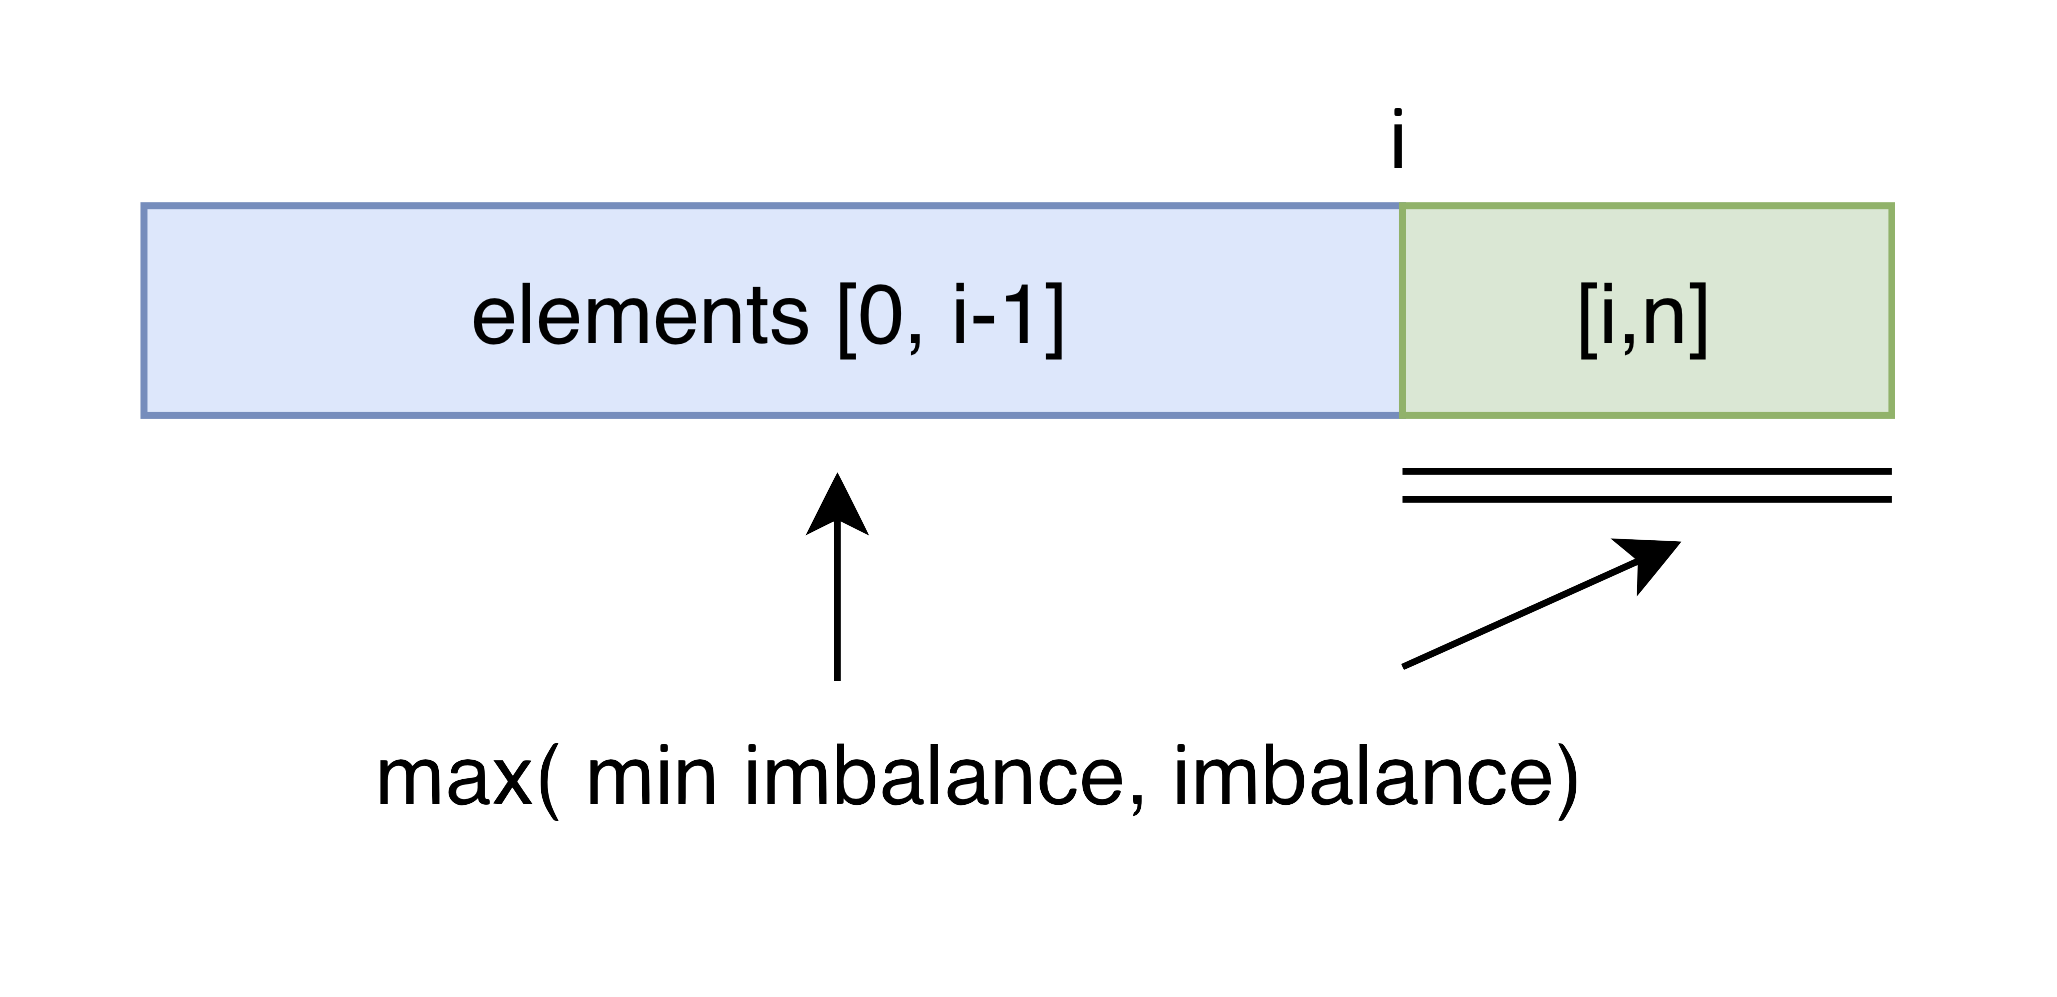
\includegraphics[width=0.4\textwidth]{Problem2Figs/CS124 PSET1_4 Diagrams.png}
    \caption{Example Placement of Partition $i$}
    \label{fig:histogram}
\end{figure}
\FloatBarrier
\subsubsection*{Recursion Equation/Explanation:}
$$\text{I[x,y]} = \underbrace{\min_{y+1 \leq i \leq x}}_{\text{(1)}} \left\{ \max \left \{ \underbrace{\left | \sum^{x}_{\ell = i} a_\ell - \text{avg} \right |}_{(2)},\ \underbrace{\text{I[i-1, y-1]}}_{(3)}\right \} \right \}$$

\begin{enumerate}
    \item This minimization tries all possible locations for this partition (within the given range and inherent limits such that the other partition can be placed---i.e., y-1 partitions need y locations to be placed because a partion cannot be place \textit{on} the first element given my definition of a partition's inclusivity (seen in Figure \ref{fig:histogram}).
    \item This absolute value of a summation minus the average uses the provided definition of imbalance to find the imbalance (from elt. $i$ to $x$) on the \enquote{right} of the current placed partition.
    \item The call to I[i-1,y-1] recursively returns the minimal imbalance setup for placing $y-1$ partitions in elements $0$ to $i-1$.
\end{enumerate}

\subsubsection*{Tracking Partitions:}
To track partitions, we'll create a size $k$ 1-D array, partitions[k], initialized to $\infty$ which we populate as follows: \\
Alongside the selection of minimum $i$ placement, we'll update partition[y] = $i-1$.  The added minus one is due to the setup of our recursion which experiences an off-by-one error with regard to the problem's definition of partitions and their left-wise inclusion, so we can easily resolve the semantical issue by decrementing the \enquote{actual} partition location by 1.

\subsubsection*{Base case:}
Our base case occurs with \textbf{I[x,0]} (i.e., no more partitions left to place).  In this case, we establish the following:
$$\text{I}[x,0] \equiv \left | \sum^{x}_{i=0} a_i\right |$$


There is never a scenario---given correct initial setup and our index limits for the iterations of \enquote{min}---wherein $x \leq y$, so we do not treat such a scenario.

\subsection{Analysis:}
\subsubsection*{Space complexity:}
We fill an $n$ by $k$ array, I, and a 1-D array of size $k$ $\implies$ \\
\rule{\textwidth}{0.4pt}
$$\mathbf{O(nk)}$$
\rule{\textwidth}{0.4pt}

\subsubsection*{Run-time:}
Given our \enquote{min} iteration, we take $n$ trials per entry of array I, so given the size of I is $nk$, we can model our time complexity:\\

\rule{\textwidth}{0.4pt}
$$\mathbf{O(n^2k)}$$
\rule{\textwidth}{0.4pt}

\subsection{Proof of correctness:}
Because our algorithm is based on recursion, we can assume correctness by merit of our definitions of base case and the recursion, itself, by induction. \\

Considering our \textbf{base case}, given a placement of no partitions, the \enquote{imbalance} of the elements up to x is just that as defined by the provided imbalance equation. \\

\textbf{Next}, placing the next partition (i.e., the only partition up to this point) splits the array into two, given the elements afforded (up to $x$), so and we now calculate the max of the imbalance of our base case versus the imbalance of the \enquote{right-side} for each eligible location of the placement of our partition, selecting the situation with the minimum maximum imbalance on either side.  This is definitionally correct given the intention of our algorithm, and is what upon which our recursion continually predicates $\implies$ correctness via induction.

\subsection{Changed Algorithm:}

Given a redefinition of imbalance, our space and time complexity do not change because we still need to check all eligible placements of each partition and select the minimum imbalance.

\subsubsection*{Re-written Recursion:}
$$\text{I[x,y]} = \min_{y+1 \leq i \leq x} \left\{ \left | \sum^{x}_{\ell = i} a_\ell - \text{avg} \right | + \text{I[i-1, y-1]}\right \}$$









\newpage



\section{Blanket for a Tree}
%%%%%%%%%%%%%%%%%%
%   Question #3  %
%%%%%%%%%%%%%%%%%%

\subsection{Setup:}
First, given a tree of size |V|, let us run a depth first search (one time cost of O(|V| + |E|) which is within our bounds because |E| = |V|-1 for a tree) to create a \enquote{pseudo-directedness} such that we can establish an leveled list of vertices based on visit order (we can start at any node on the tree).  This affords an arrangement such that we can traverse the list of vertices and find \enquote{children} on the previously undirected tree by finding edges shared between a vertex, $v_{parent}$ and vertices $v_j$, the latter of which are at a higher index in the list of vertices.

\subsection{Definition:}
B[i, boolean] returns the minimum blanket size of a subtree starting at \enquote{root} $i$ given whether the root itself is included (which predicates whether its children must or must not be included) or not included (i.e., the boolean input).  The subtree is well-defined because of our initial DFS ensures a logical ordering to our vertices 

\subsubsection*{Where to find our answer?}
Simply find the minimum of B[0, true] or B[0, false] to find the minimum blanket size.\\
Additionally, check the vector containing best vertices included in the blanket---see more in Section \ref{theBlanket}.

\subsection{Recursion:}
Notation: $v_c \in (v, u)$ where the indices of $u$ are greater than that of $v$ regarding the prior DFS sorted list.

\subsubsection{Attempt 1:}
Blanket[v] = 
$\begin{cases}
    \begin{cases}
        \sum^{}_{v_j \in v_c} \text{Blanket[c]}, & \textbf{if } \text{ALL children included up to this point}\\
        1 + \sum^{}_{v_j \in v_c} \text{Blanket[c]}, & \textbf{otherwise}\\
    \end{cases}\\ \\
    0 & \textbf{if } \text{no children}
\end{cases}$

\subsubsection{Attempt 2:}
We need to be able to recur by choosing a case, which requires knowing if the children are on or off, so we can choose to keep two scenarios which does not harm our space complexity as we multiply our 2 (not hugely problematic).  As a side note regarding \textbf{space complexity}, we can see that we store a list of vertices of size |V| and a list of minimum blanket sizes for a subtree covered by the blanket corresponding to each selected vertex, which requires another two arrays of size |V| (one for if the vertex is included; one for not included).  This is clearly \textbf{O(|V|)} space. \\

\textbf{Our equations, then:} \\
$$\text{B[v, false]} = \sum^{}_{j \in v_c}\text{B[$v_j$, true]}$$
$$\text{B[v, true]} = 1 + \sum^{}_{j \in v_c}\min(\text{B[$v_j$, false]}, \text{B[$v_j$, true]})]$$

This is true because considering the subtree must take the children of vertex $v$ if it is not itself included to ensure that all its edges to its children are covered.  Else, if vertex $v$ is included, we need not always take its children unless that's the best setup for them (minimal).

\subsubsection{Base case:}
Now using attempt 2, we establish a base case where if a vertex, $v$, has no children (i.e., edges to other nodes further \enquote{right} (higher index) in the sorted list populated by our initial DFS), then we assign the following values to its corresponding entries in each B-array: \\
$$\text{B}[v_{\text{no children}}, \text{false}] \coloneq 0$$
$$\text{B}[v_{\text{no children}}, \text{true}] \coloneq 1$$

\subsubsection{The actual blanket:} \label{theBlanket}
At each iteration where we check both B[v, false] and B[v, true], we can populate an additional vector (to which we can append, but will not exceed size |V|) with the vertex itself \textbf{iff} B[v, true] > B[v, false].  This way, we can find the actual blanket when after we run both B[1, true] and B[1, false] by simply checking which vertices are in this repeatedly appended-to vector.

\subsection{Proof of correctness:}
Because our algorithm is based on recursion, we can assume correctness by merit of our definitions of base case and the recursion, itself, by induction. \\

The base case is handled correctly, as a node with no children and dependent on a boolean of inclusion (true, false) returns a blanket size of 1 if included or 0 if not.\\

Moving up to a \textbf{next step}, we know that if a parent is not taken (false), then we must take the children (who have no children) which returns correctly a blanket of size |children| covering the shared edges.  Else, if we do take the parent, we can choose whether or not to take the children (who have no children)---whichever is minimal---so our recursion will choose \textit{not} to take the children, and so our blanket size is 1, just the parent, which still covers all edges (to children--because they have no children), and we'd pick the minimum of the two options if this were the actual \enquote{pseudo-root} of the entire graph as sorted by the DFS $\implies$ we select the parent on and children off, which is, correctly, the cheapest/minimal blanket cover.

\subsection{Analysis:}
\subsubsection*{Space complexity:}
As mentioned above, we need an array to order the vertices and two arrays for situations where either a vertex is included or not included and its ensuing minimal blanket size from that node as the root down through its subtree. \\

These are all of size |V|, so we can take \textbf{O(|V|)}

\subsubsection*{Run-time:}

We know the Depth First Search, run once is O(|V|).  For each array, B[don't care, FALSE] and B[don't care, TRUE], we recur down through children which inevitably each a base case of two-operations (note that because this is a tree $\implies$ no cycles, so vertices are \textbf{not} re-visited, and we populate an array (bottom-up/back-to-front) as we pop back up with a similar constant time comparison for each) which is O(2|V|) at worst per column of the array enumerated above $\implies$ \textbf{O(|V|)}.






\newpage

\section{Buffy's Word Processor (Printing Neatly)}
%%%%%%%%%%%%%%%%%%
%   Question #4  %
%%%%%%%%%%%%%%%%%%
\subsection{Definition:} \label{D-arrayDef}
For Buffy's printing problem, let \textbf{D[i,k]} be the best case penalty (an integer value) for an arrangement of line-breaks on a paragraph with words $\ell_i$ to $\ell_n$ wherein any number of line breaks can be placed only \textbf{after} word $\ell_k$, and $n$ is the total number of words in the paragraph.

Our lookup table, \textbf{D[i,k]} is an $n$ by $n$ array which is filled from cell $(n,n)$ up. (Specifically, it fills an upper triangular portion of the LUT reverse column by column filling $(n,n) \rightarrow (n-1, n)$ and so on.

\rule{\textwidth}{0.4pt}
\subsubsection*{Where's our answer?}
To find our answer, we would look in cell $D[0,0]$ which returns the best case penalty for our paragraph whereby any line-breaks are eligible to be placed after the first word. \\
\rule{\textwidth}{0.4pt}

\subsection{Recursion:}
\subsubsection{Penalty Function:} \label{penaltyfunc}
To easily find costs and establish some base cases we define:

$$\mathbf{f(i,k)}=\begin{cases}
   \ 0 & \textbf{if } k=n \textbf{ and } (k-i + \sum^{k}_{a = i} \ell_a) < M  \\
    \ \infty & \textbf{if } (k-i + \sum^{k}_{a = i} \ell_a) > M \\
    \ [M-(k-i + \sum^{k}_{a = i} \ell_a)]^3 & \textbf{otherwise}
\end{cases}$$

\begin{enumerate}
    \item The first case treated is if we only allow a line break to occur after the $k$th word which happens to be the last word \textbf{and} the whole list of words $(i,k)$ fit on a line without exceeding $M$.  (Essentially, this handles the placement of our last line with no penalty.)
    \item The second case is where we try to place a number of words on a single line which exceeds our boundary, $M$, so it is essentially infinite penalty because this is undefined behavior.
    \item The third case is our general penalty calculation as delineated in the PSET spec.\\
\end{enumerate}


\subsubsection{Full Recursion:} \label{4func}
In addition to our array, D, we must store an array, B, which is $n$ by $n$ and contains tuples in each entry which are an ordered pair pointing to a next cell (the cell which provides the minimal penalty next:

$$\mathbf{D[i,k]}=\begin{cases}
    \textbf{min}
    \begin{cases}
        f(i,k) + D[(k+1), (k+1)]; & \text{B[i,k]} \coloneq (k+1, k+1) \\
        D[i,(k+1)]; & \text{B[i,k]} \coloneq (i, k+1)
    \end{cases}  & \textbf{if } k<n \\
    \ f(i,k) & \textbf{if } k \geq n
\end{cases}$$

\begin{enumerate}
    \item If $k < n$, we can try two scenarios: \begin{enumerate}
        \item Either, we can place a line-break after $\ell_k$ and continue our recursion (noting that a break-point has been placed by providing B[i,k] an ordered pair pointing to a next cell along the array's diagonal)
        \item or we can not place a line-break here and see the cost of placing one after a future word, i.e., $\ell_{k+1}$ (noting that a break-point has \textbf{not} been placed by providing B[i,k] an ordered pair inclusive of our start word index, $i$ and a future index, $k+1$).
    \end{enumerate}
    \item If $k \geq n$, we define a base-case where we assign this element our penalty function's return value, because there are no further possible placements of line-breaks, at indices $k$, after $n$ (no ordered-pair needed in B array since no next line-break).
\end{enumerate}

\subsubsection{Break-point finding:} \label{breakFind}
To locate our breakpoints, we create an array of size $n$ of \textbf{false} Boolean values which reflect whether a line-break is placed after $\ell_i$---let's call this array breaks[n].\\

For our desired output, we start in cell B[1,1] (corresponding to our least cost solution cell---D[1,1]) and refer to our assignments from the full-recursion listing.  \textbf{If} we see each value of the tuple held at B[1,1] equal one another, by our full-recursion structure, we know that a line break should go after this element, so we update breaks[1] to a \textbf{true} boolean value which we will use when printing (see more detailed setup in code section \ref{code:printing}).  \textbf{Otherwise,} we update leave breaks[1] as \textbf{false} and move to the next entry of array B as indicated by the ordered-pair stored at B[1,1].  Continuing this process $n$ times, can fully update the breaks[n] array with locations of penalty-minimizing line-breaks.
    
\subsection{Analysis:}
\subsubsection*{Space complexity:}
We fill an $n$ by $n$ matrix D with penalties, an $n$ by $n$ matrix B with tuple-pointers to reconstruct line-break location (we can model this as 2 $n$ by $n$ matrices), and a size $n$ 1-D array of Boolean values for printing/cleanly returning line-breaks.\\
\rule{\textwidth}{0.4pt}
$$\mathbf{O(n^2)}$$
\rule{\textwidth}{0.4pt}

\subsubsection*{Run-time:}
There exists constant time work to fill each element of the array (additions based on prior array elements and our penalty function) (we do not re-touch elements, either), and we fill $n^2$ elements $\implies$ \\
\rule{\textwidth}{0.4pt}
$$\mathbf{O(n^2)}$$
\rule{\textwidth}{0.4pt}


\subsection{Proof of correctness:}
Because our algorithm is based on recursion, we can assume correctness by merit of our definitions of base case and the recursion, itself, by induction. \\

\textbf{Base case:} for \textbf{D[i,k]} where $k \geq n$ we define $D[i,k] = f(i,n)$ (see Section \ref{4func}).  By our definition of the array D and what its indices represent (see Section \ref{D-arrayDef}), we know that, given $k \geq n$, there are no more locations where a line-break may be placed, so we must calculate penalty for placing words $(i,n)$ on the same line (namely, the last).  If the words and their spaces cannot fit given our $M$ constraint, we assign $\infty$ penalty because the setup is not allowed; else it fits, so there is no penalty (i.e., $0$) because it is the last line.  This fills the right-most column of our array D.  Our base-case is correct by definition.

Our \textbf{next step} is based on recursion and correctly selects the minimum of \textbf{either} the penalty of putting words $i$ up to $k-1$ (let us take $k = n$ from our base case) on a line and the penalty of putting placing word $\ell_k$ on its own line (which is ignored if M is sufficiently large because it is the last line) \textbf{or} the penalty of putting $i$ up to $k$ on a single line (the last line because $k=n$) which if it fits is the better placement scenario, but if it doesn't, will return $\infty$, so then clearly the other option (break after $\ell_{k-1}$) is selected correctly.


\subsection{Code:}
\subsubsection*{Initialization Steps:}
\begin{minted}{python}
    import numpy as np
    
    text_file = open("buffy.txt", "r")
    lines = text_file.read().split()
    text_file.close()
    
    M = 40                  # input parameters
    M2 = 72
    n_words = len(lines)    # number of words
\end{minted}

\subsubsection*{Cost Function:}
The following implements our penalty function from Section \ref{penaltyfunc}.
\begin{minted}{python}
    def penalty(i,k):
        summed = 0
        if (i == k):                 # python indexing issue resolution
            summed = len(lines[i])
        else:
            for j in range (i,k+1):
                summed += len(lines[j])
          
        if ((k == n_words-1) and ((k-i+summed) < M)):
            return 0
            
        elif ((k-i+summed) > M):
            return float("inf")
        
        else:
            return ((M-(k-i + summed))**3)
\end{minted}

\subsubsection*{Array Initialization:}
\begin{minted}{python}
    D = np.empty([len(lines), len(lines)]) # best penalty given [i,k] parameters
    B = np.empty([len(lines), len(lines)]) # x-coord. next best cell (break tracking)
    C = np.empty([len(lines), len(lines)]) # y-coord. next best cell (break tracking)
\end{minted}

    
\subsubsection*{Array Filling:}
Though not shown as a recursive function, the following effectively refers to prior elements in the look-up table to populate bottom-up.  It matches the algorithm described in Section \ref{4func}.
\begin{minted}{python}
    for k in range((n_words-1), -1, -1):
        for i in range (k,-1,-1):
            if(k >= n_words-1):         # base case
                D[i,k] = penalty(i,k)
            else:
                # find minimum
                if (penalty(i,k) + D[k+1, k+1]) < D[i,k+1]:
                    B[i,k] = k+1
                    C[i,k] = k+1
                    D[i,k] = (penalty(i,k) + D[k+1, k+1])
                else:
                    B[i,k] = i
                    C[i,k] = k+1
                    D[i,k] = D[i,k+1]
\end{minted}


\subsubsection*{Break-Point Finding (and printing):}
The following implements the procedure outlined in Section \ref{breakFind}:
\begin{minted}{python}
    breaks = np.zeros((n_words,1)) # bool for whether we break after word i

    # initialize our location (treating as ordered pair)
    x = 0 
    y = 0
    for i in range (0,n_words):
        x = int(x) # python-specific data cleaning
        y = int(y) # python-specific data cleaning
        if B[x,y] == C[x,y]:  # i.e., we added a break
                              # (penalty(i,k) and called D[k+1, k+1])
            breaks[i] = 1     # so break after this word
        old_x = x
        
        # get the ordered pair for our next location to check for line-break
        x = B[x,y]
        y = C[old_x,y]
\end{minted}


\subsection{Results:}
\subsubsection*{M = 40}
\textbf{Penalty = 2183} \\
\textbf{Printed text}:\\
\rule{\textwidth}{0.4pt}
\begin{minted}{text}
    Buffy the Vampire Slayer fans are 
    sure to get their fix with the DVD 
    release of the show's first season. 
    The three-disc collection includes all 
    12 episodes as well as many extras. 
    There is a collection of interviews 
    by the show's creator Joss Whedon in 
    which he explains his inspiration for 
    the show as well as comments on the 
    various cast members. Much of the same 
    material is covered in more depth with 
    Whedon's commentary track for the show's 
    first two episodes that make up the 
    Buffy the Vampire Slayer pilot. The 
    most interesting points of Whedon's 
    commentary come from his explanation 
    of the learning curve he encountered 
    shifting from blockbuster films like Toy 
    Story to a much lower-budget television 
    series. The first disc also includes 
    a short interview with David Boreanaz 
    who plays the role of Angel. Other 
    features include the script for the 
    pilot episodes, a trailer, a large photo 
    gallery of publicity shots and in-depth 
    biographies of Whedon and several of the 
    show's stars, including Sarah Michelle 
    Gellar, Alyson Hannigan and Nicholas 
    Brendon. 
\end{minted}
\rule{\textwidth}{0.4pt}

\newpage
\subsubsection*{M = 72}
\textbf{Penalty = 2104} \\
\textbf{Printed text}:\\
\rule{\textwidth}{0.4pt}
\begin{minted}{text}
Buffy the Vampire Slayer fans are sure to get their fix with the DVD 
release of the show's first season. The three-disc collection includes 
all 12 episodes as well as many extras. There is a collection of 
interviews by the show's creator Joss Whedon in which he explains 
his inspiration for the show as well as comments on the various cast 
members. Much of the same material is covered in more depth with 
Whedon's commentary track for the show's first two episodes that make 
up the Buffy the Vampire Slayer pilot. The most interesting points of 
Whedon's commentary come from his explanation of the learning curve 
he encountered shifting from blockbuster films like Toy Story to a 
much lower-budget television series. The first disc also includes a 
short interview with David Boreanaz who plays the role of Angel. Other 
features include the script for the pilot episodes, a trailer, a large 
photo gallery of publicity shots and in-depth biographies of Whedon and 
several of the show's stars, including Sarah Michelle Gellar, Alyson 
Hannigan and Nicholas Brendon. 
\end{minted}
\rule{\textwidth}{0.4pt}


\end{document}
